\section{Constrained optimisation and Lagrange
 multipliers}
\subsection{Lagrange multipliers}
One often needs to maximise or minimise a function subject to certain
constraints.
 
\begin{center}
\fbox{\begin{minipage}{7in}
\begin{example}
Find the minimum value of \( x^2 + y^2 \) subject to the constraint \( x+y
 = 1 \).
\\\\
We want to minimise the function \( f \)subject to the constraint \( x+y = 1 \)
\\\\
We can explicitly solve the \textbf{constraint-equation:} \( y = 1-x\), so
\[ 
   F(x) := f(x,1-x) = x^2 + (1-x)^2 = 2x^2 - 2x+1
\]
Which is a function of \( x \) alone. The critical points of \( F \) occur when
\( F'(x) = -2+4x = 0 \), implying \( x = \frac{1}{2} \). Since \( F''(x)
= 4 > 0 \), it follows that \( F \) has a minimum at \( x = \frac{1}{2}
\). Therefore \( f \) subject to the constraint \( x+y = 1 \) achieves its
minimum value at \( x = y = \frac{1}{2} \) with the actual value also \(
\frac{1}{2} \).
\\\\
You can solve this problem much better without requiring the explicit solution
of the constraint-equation.
\\\\
Define a second function \( g \) such that the constraint-equation corresponds
to \( g(x,y) = 0 \). % Apply more clarity later.
 
In our example, \( g(x,y) = x + y - 1 \). Graphing the contour polot \( f(x,y)
= x^2 + y^2\) and add a graph of the single contour \( g(x,y) = 0 \).
\end{example}
\end{minipage}}
\end{center}


\begin{figure}[h]
  \centering
  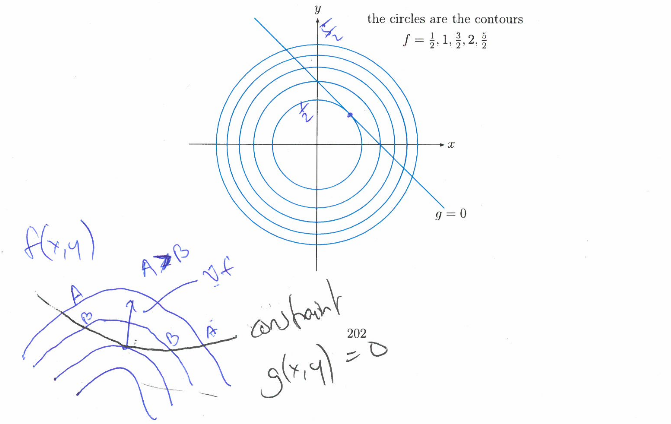
\includegraphics[width=0.6\linewidth]{./lectures/DeepinScreenshot_select-area_20191013194637}
  \caption{}%
  \label{}
\end{figure}

The minimum occurs where the contour \( g(x,y) = 0 \) touches one of the
contours of \( f \), which means that \( \nabla f \) and \( \nabla g \) are
parralel. Hence

\[ 
  \nabla f = \lambda \nabla g
\]
for some \( \lambda \), known as the \textbf{Langrange multiplier}.

\begin{center}
\fbox{\begin{minipage}{7in}
\begin{example}
Find the minimum value of \( x^2 + y^2 \) subject to the constraint \( x+y = 1 \)
\\\\
Let \( f(x,y) = x^2 + y^2 \) and \( g(x,y) = x+y-1 \). We want to minimise \(
f(x,y)  \) subject to the constraint \( g(x,y) = 0 \). Next, \( \nabla
f = (2x,2y) \) and \( \nabla g = (1,1) \). Set \( \nabla f = \lambda \nabla
g \), so \( 2x = \lambda \), \( 2y = \lambda \). Including the constraint \(
g(x,y) = 0 \), this gives us 3 equations in 3 unknowns. The solution is \(
x = y = \frac{1}{2} \), \( \lambda = 1 \). To verify that this is a minimum,
set \( x = \frac{1}{2} + \varepsilon \), \( y = \frac{1}{2}- \varepsilon \)
such that \( x + y = 1 \).
\begin{align*}
  f( \frac{1}{2} + \varepsilon, \frac{1}{2} - \varepsilon) &= \Big( \frac{1}{2}
  + \varepsilon\Big)^2 + \Big( \frac{1}{2} - \varepsilon \Big )^2 \\
  &= \frac{1}{2} + 2 \varepsilon^2
\end{align*}
We see that \( f( \frac{1}{2} + \varepsilon, \frac{1}{2} - \varepsilon) \) is
minimised when \( \varepsilon = 0 \), so (\( \frac{1}{2}, \frac{1}{2} \)) gives
the constrained minimum.
\end{example}
\end{minipage}}
\end{center}

\begin{note}
The following two remarks are important and are direct references to the
workbook.
\end{note}

\begin{remark}
When solving a constrained optimisation problem with Langrange multipliers, it
is typically not necessary to find the value of \( \lambda \). So when solving
your equations obtained from \( \nabla f = \lambda \nabla g\) and the
constraint-equation, your aim is really to \textbf{eliminate} \( \lambda \) in
order to solve for variables in your problem. \\\\
If upon using the method of Langrange multipliers you obtain simple, linear
equations to solve then consider yourself lucky. In some cases you will in fact
obtain nonlinear equations that you need to solve. If this happens we suggest
the first thing you to is try taking the \textbf{ratio} of your equations
obtained from \( \nabla f = \lambda \nabla g \). This allows you to immediately
eliminate \( \lambda \) from your equations and proceed from there. The next
example nicely illustrates this point.
\end{remark}



